\section{Resultados}\label{sec:resultados}

\subsection{Primer experimento: Comprobaci�n de que los tres rayos
involucrados y la normal est�n en el mismo plano}\label{subsec:primero}

\subsection{Segundo experimento: Medida de los �ngulos de reflexi�n y refracci�n}\label{subsec:segundo}

\begin{table}[h!]
    \center
    \caption{�ngulos de incidencia $\theta_i$, de reflexi�n $\theta_r$ y de refracci�n $\theta_t$.}
    \label{tab:radio}
    \begin{centering}
        \begin{tabular}{|P{40px}|P{40px}|P{40px}|}
            \hline
            $\theta_i\,$(\textdegree) & $\theta_r\,$(\textdegree) & $\theta_t\,$(\textdegree)              \\
            \hline
            \csvreader[late after line= \\, /csv/separator=semicolon ]{./files/data/segundo_es.csv}{}% use head of csv as column names
            {\csvcoli                 & \csvcolii                 & \csvcoliii    }% specify your columns here
            \hline
        \end{tabular}
    \end{centering}
\end{table}


\begin{figure}[tbh]
    \begin{center}
        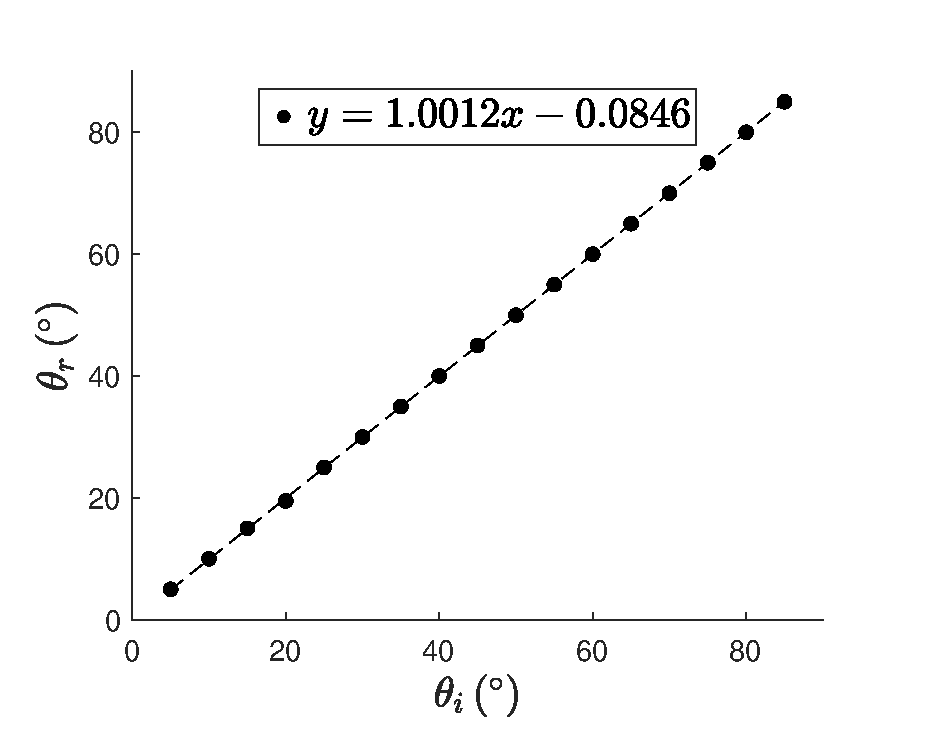
\includegraphics[width=0.8\columnwidth]{files/images/reflexion}
    \end{center}
    \caption{�ngulo de reflexi�n $\theta_r$ frente al �ngulo de incidencia $\theta_i$.}
    \label{fig:reflexion}
\end{figure}

\begin{figure}[tbh]
    \begin{center}
        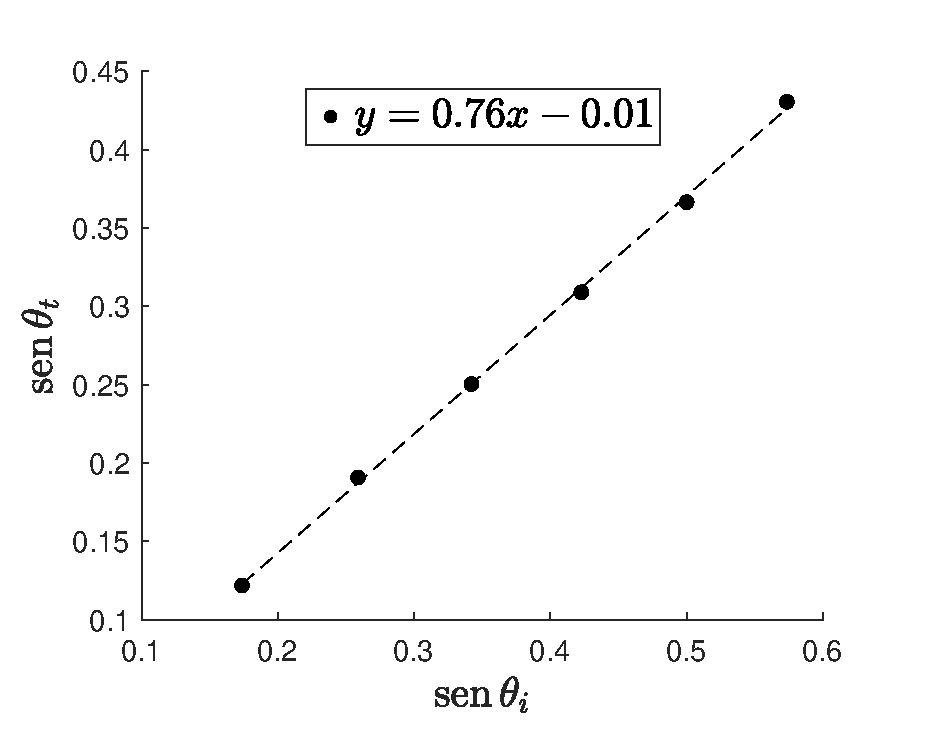
\includegraphics[width=0.8\columnwidth]{files/images/refraccion}
    \end{center}
    \caption{Seno del �ngulo de refracci�n $\theta_t$ frente al seno del �ngulo de incidencia $\theta_i$.}
    \label{fig:refraccion}
\end{figure}


\begin{figure}[tbh]
    \begin{center}
        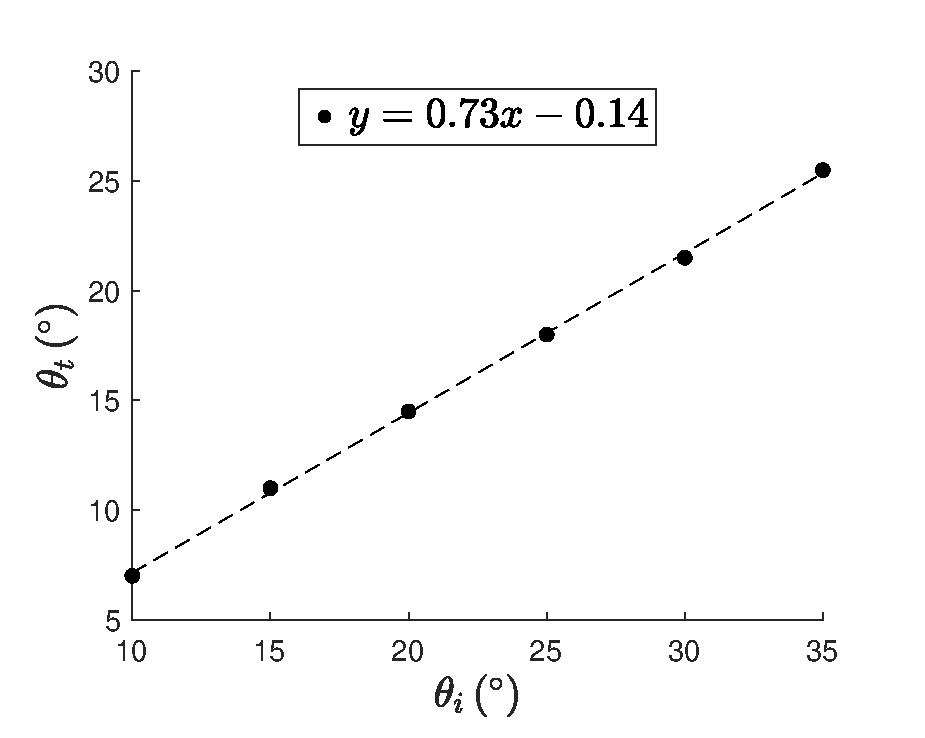
\includegraphics[width=0.8\columnwidth]{files/images/aproximacion}
    \end{center}
    \caption{�ngulo de refracci�n $\theta_t$ frente al �ngulo de incidencia $\theta_i$.}
    \label{fig:aproximacion}
\end{figure}

\FloatBarrier

\subsection{Tercer experimento: �ngulo l�mite}\label{subsec:tercero}


\begin{table}[h!]
    \center
    \caption{�ngulos de incidencia $\theta_i$ desde el agua en torno al �ngulo l�mite.}
    \label{tab:limite}
    \begin{centering}
        \begin{tabular}{|P{40px}|P{60px}|P{60px}|}
            \hline
            $\theta_i\,$(\textdegree) & Transmisi�n & No transmisi�n                         \\
            \hline
            \csvreader[late after line= \\, /csv/separator=semicolon ]{./files/data/limite.csv}{}% use head of csv as column names
            {\csvcoli                 & \csvcolii   & \csvcoliii    }% specify your columns here
            \hline
        \end{tabular}
    \end{centering}
\end{table}
